
\def\dX{6.0}
\def\dY{3.0}

  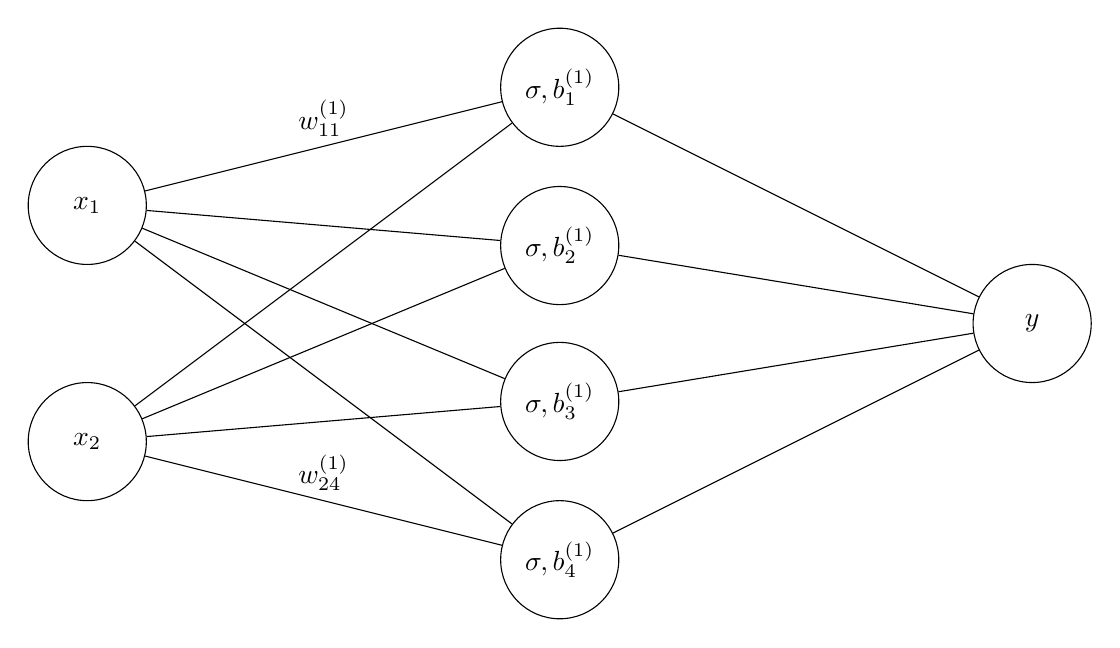
\begin{tikzpicture}
    %%   (lable)  (x, y)     {\text}
    \node[shape=circle,draw=black, minimum size=1.5cm] (X1) at (-\dX,  0.50*\dY) {$x_1$};
    \node[shape=circle,draw=black, minimum size=1.5cm] (X2) at (-\dX, -0.50*\dY) {$x_2$};
    \node[shape=circle,draw=black, minimum size=1.5cm] (Y)  at (+\dX,         0) {$y$};

    \node[shape=circle,draw=black, minimum size=1.5cm] (N1) at (0,      \dY) {$\sigma,b_1^{(1)}$};
    \node[shape=circle,draw=black, minimum size=1.5cm] (N2) at (0, 0.33*\dY) {$\sigma,b_2^{(1)}$};
    \node[shape=circle,draw=black, minimum size=1.5cm] (N3) at (0,-0.33*\dY) {$\sigma,b_3^{(1)}$};
    \node[shape=circle,draw=black, minimum size=1.5cm] (N4) at (0,     -\dY) {$\sigma,b_4^{(1)}$};

    \path[-] (X1) edge node[above] {$w_{11}^{(1)}$} (N1);
    \path[-] (X1) edge                              (N2);
    \path[-] (X1) edge                              (N3);
    \path[-] (X1) edge                              (N4);
    %
    \path[-] (X2) edge                              (N1);
    \path[-] (X2) edge                              (N2);
    \path[-] (X2) edge                              (N3);
    \path[-] (X2) edge node[above] {$w_{24}^{(1)}$} (N4);

    \path[-] (N1) edge (Y);
    \path[-] (N2) edge (Y);
    \path[-] (N3) edge (Y);
    \path[-] (N4) edge (Y);

  \end{tikzpicture}
